\section{Pulse Processing Electronics}
{\color{red} This section still needs to be done!!!}
\subsection{General Concepts}
\begin{itemize}
    \item In the context of this course, signal amplification and shaping is done in analog then converted to digital  
    \item As shown in figure~\ref{fig:signal_processing}, the signal processing and pulse-shape system goes as the following:\\
    An incident radiation interacts in the detector and deposits energy as a current pulse that is usually too small to be measured directly. The current is therefore sent to the preamplifier, which integrates the transient current pulse to produce a voltage step that is proportional to the pulse. The shaping amplifier then converts the output of the preamplifier into a form suitable for measurements, producing an output voltage pulse with its pulse height proportional to the initial deposited charge. 
\end{itemize}
\begin{figure}[ht]
    \centering
    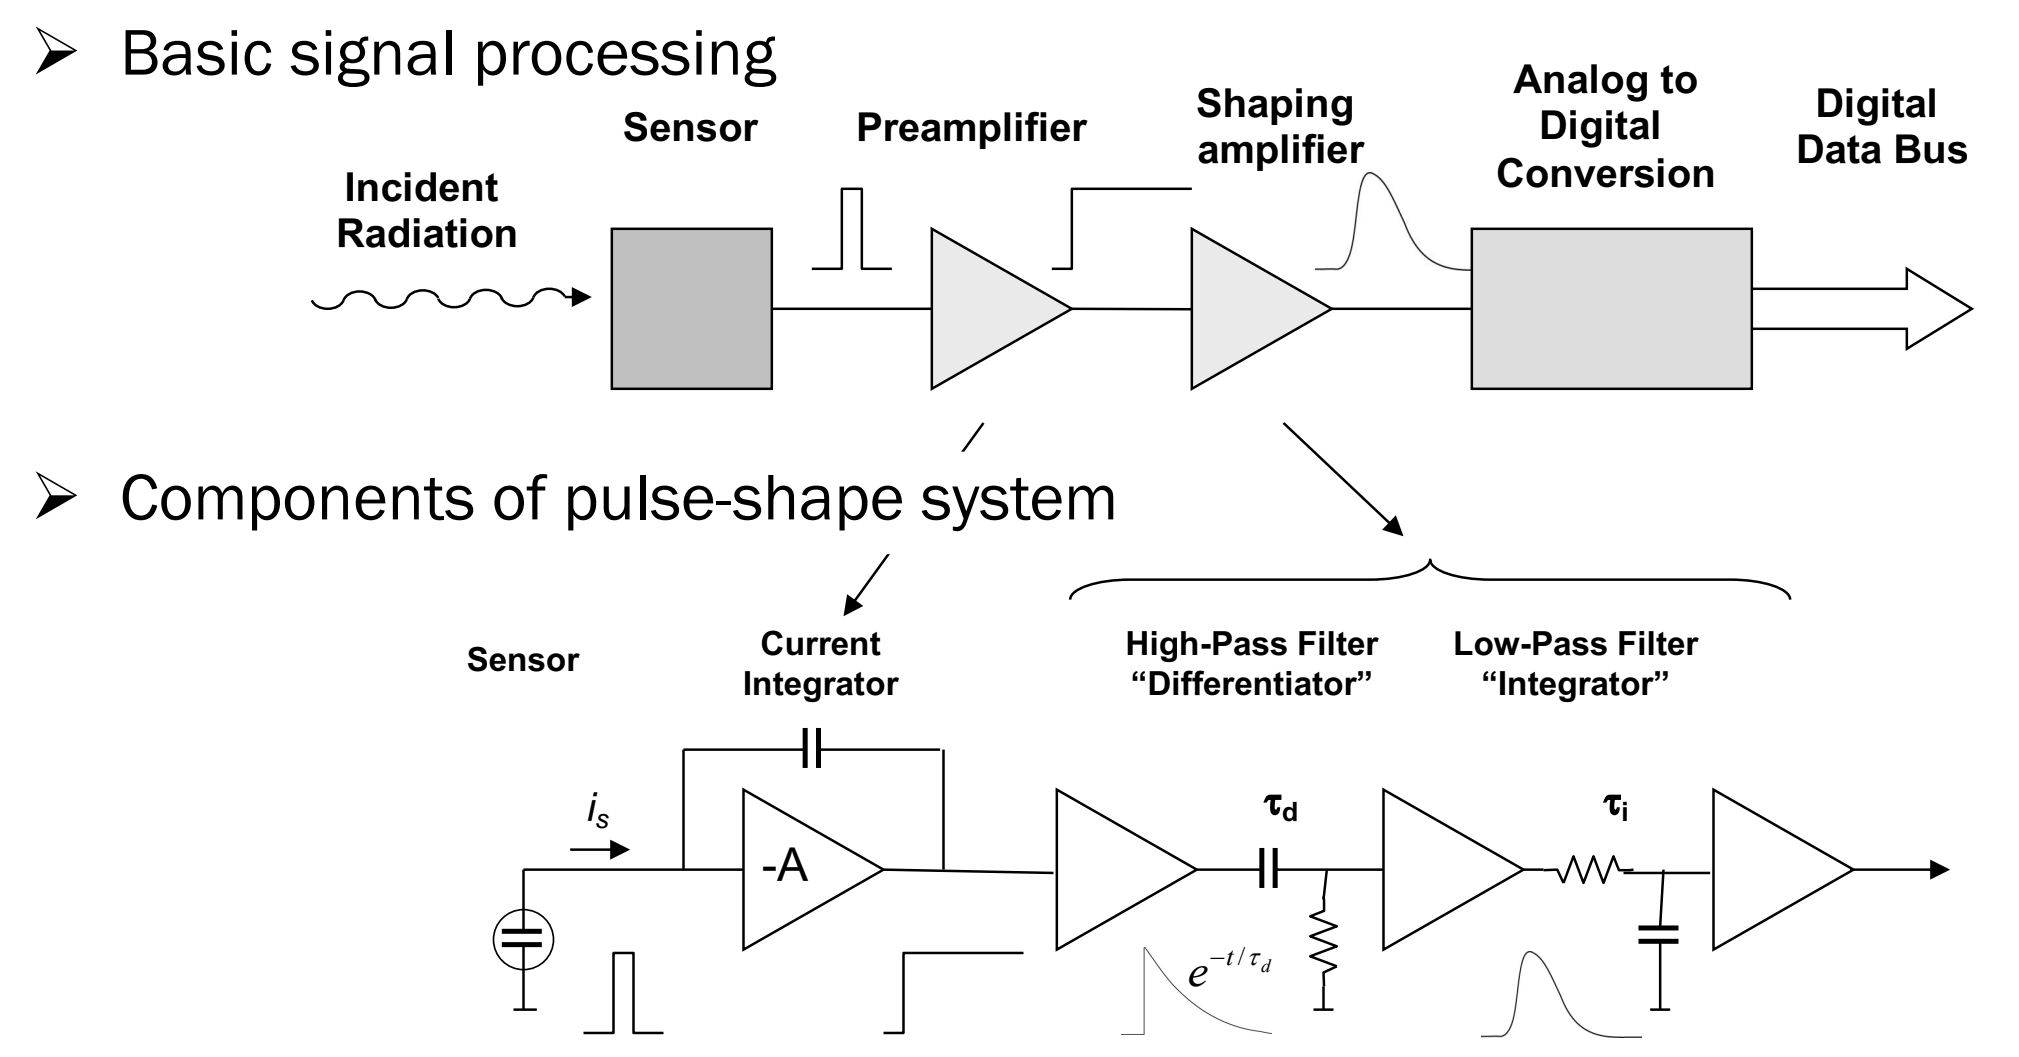
\includegraphics[width=0.8\textwidth]{images/signal_processing_diagram.png}
    \caption{Signal processing diagram.}
    \label{fig:signal_processing}
\end{figure}
\subsection{Components}
\subsubsection{Preamplifier}
\begin{figure}[ht]
    \centering
    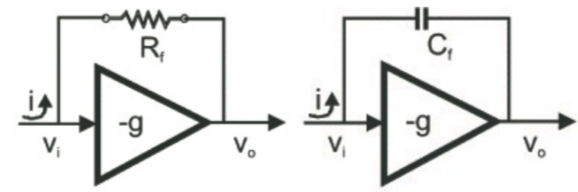
\includegraphics[width=0.45\textwidth]{images/preamp_circuit_current_charge.png}
    \caption{Circuits of the current (left) and charge (right) sensitive preamplifiers.}
    \label{fig:preamp_circuit_current_charge}
\end{figure}
\begin{figure}[ht]
    \centering
    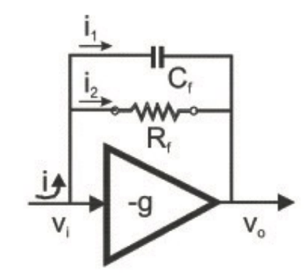
\includegraphics[width=0.25\textwidth]{images/preamp_circuit_resistive_feedback.png}
    \caption{Circuit of the resistive feedback preamplifier.}
    \label{fig:preamp_circuit_resistive_feedback}
\end{figure}
\begin{enumerate}
    \item General function:
    \begin{itemize}
        \item Convert charge to voltage
        \item Amplifies a signal with minimal noise
        \item Matches the high detector impedance to the low impedance of amplifier input
        \item Filters very low frequencies
    \end{itemize}
    \item Current-sensitive preamplifier, see figure~\ref{fig:preamp_circuit_current_charge} (left):
    \begin{itemize}
        \item[] The op-amp gives $V_o=-gV_i$
        \item[] $iR_f=V_i-V_o$
        \item[] $V_o-\frac{iR_f}{1+1/g}\approx-iR_f$
    \end{itemize}
    \item Charge-sensitive preamplifier, see figure~\ref{fig:preamp_circuit_current_charge} (right):
    \begin{itemize}
        \item[] $q=\int_0^ti\;dt'=C_f(V_i-V_o)$
        \item[] $V_o=-\frac{q}{C_f(1+1/g)}\approx-\frac{q}{C_f}$
    \end{itemize}
    \item Resistive feedback preamplifier, see figure~\ref{fig:preamp_circuit_resistive_feedback}:
    \begin{itemize}
        \item[] $V_i-V_o=-V_o(1+1/g)=\int_0^t\frac{i_1}{C_f}dt'=i_2R_f$
        \item[] $i=i_1+i_2=-C_f(1+1/g)\frac{dV_o}{dt}-(1+1/g)V_o/R_f$
        \item[] $\Rightarrow\; \frac{dV_o}{dt}+\frac{1}{\tau}V_o=\frac{-i}{C_f(1+1/g)}$ , $\tau=R_fC_f$
        \item[] $\Rightarrow$ For $i(t')=-q\delta(t')$, $V_0=-\frac{qe^{-t/\tau}}{C_f(1+1/g)}$ , $\tau\gg t_\text{collection}$
        \item These preamplifiers are limited by pile-up and additional noise due to $R_f$; an alternative would be pulsed-reset preamplifiers.
        \item Preamplifier gain is given by $V_{out}/q_{in}$, in units of $[V/pC]$;\\
        $V_{out}$ is measured at the peak of the pulse.
    \end{itemize}
\end{enumerate}
\subsubsection{Shaping or Linear Amplifier}
\begin{enumerate}
    \item General function:
    \begin{itemize}
        \item 
    \end{itemize}
    \item Pulse-processing
    \begin{enumerate}
        \item CR circuit (differentiator, HPF), see figure~\ref{fig:RC_CR_circuits} (left):
        \begin{itemize}
            \item[] $V_{in}=Q/C+V_{out}$
            \item[] $\frac{dV_{in}}{dt}=\frac{1}{C}\frac{dQ}{dt}+\frac{dV_{out}}{dt}$
            \item[] With $i=\frac{dQ}{dt}=\frac{V_{out}}{R}$ and $\tau=RC$
            \item[] $V_{out}+\tau\frac{dV_{out}}{dt}=\tau\frac{dV_{in}}{dt}$
            \item For small $\tau$ (fast electronics), $V_{out}\approx\tau\frac{dV_{in}}{dt}$\\
            The differentiator removes low frequency components and is called a high-pass filter.
            \item For large $\tau$ (slow electronics), $\tau\frac{dV_{out}}{dt}\approx\tau\frac{dV_{in}}{dt}$, $V_{out}\approx V_{in}$
        \end{itemize}
        \item RC circuit (integrator, LPF), see figure~\ref{fig:RC_CR_circuits} (right):
        \begin{itemize}
            \item[] $V_{in}=iR+V_{out}$
            \item[] With $i=\frac{dQ}{dt}=C\frac{V_{out}}{dt}$ and $\tau=RC$
            \item[] $V_{in}=\tau\frac{dV_{out}}{dt}+V_{out}$
            \item For small $\tau$ (fast electronics), $V_{out}\approx V_{in}$
            \item For large $\tau$ (slow electronics), $\frac{V_{in}}{\tau}\approx \frac{dV_{out}}{dt}\;\Rightarrow\;\frac{1}{\tau}\int V_{in}dt\approx V_{out}$\\
            The integrator removes high frequency components and is called a low-pass filter.
        \end{itemize}
        \item 
    \end{enumerate} 
\end{enumerate}
\begin{figure}[ht]
    \centering
    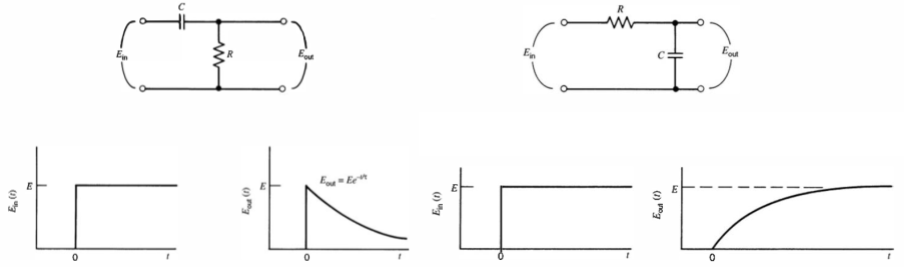
\includegraphics[width=1.0\textwidth]{images/RC_CR_circuits.png}
    \caption{The CR (left) and RC (right) circuits.}
    \label{fig:RC_CR_circuits}
\end{figure}

\subsubsection{Other Components}

\subsection{Measurements of Interest}
\subsubsection{Energy Measurement}
\subsubsection{Time Measurement}